\section{Графический интерфейс}
Приведем пример работы.\\
\begin{figure}[h!]
\begin{center}
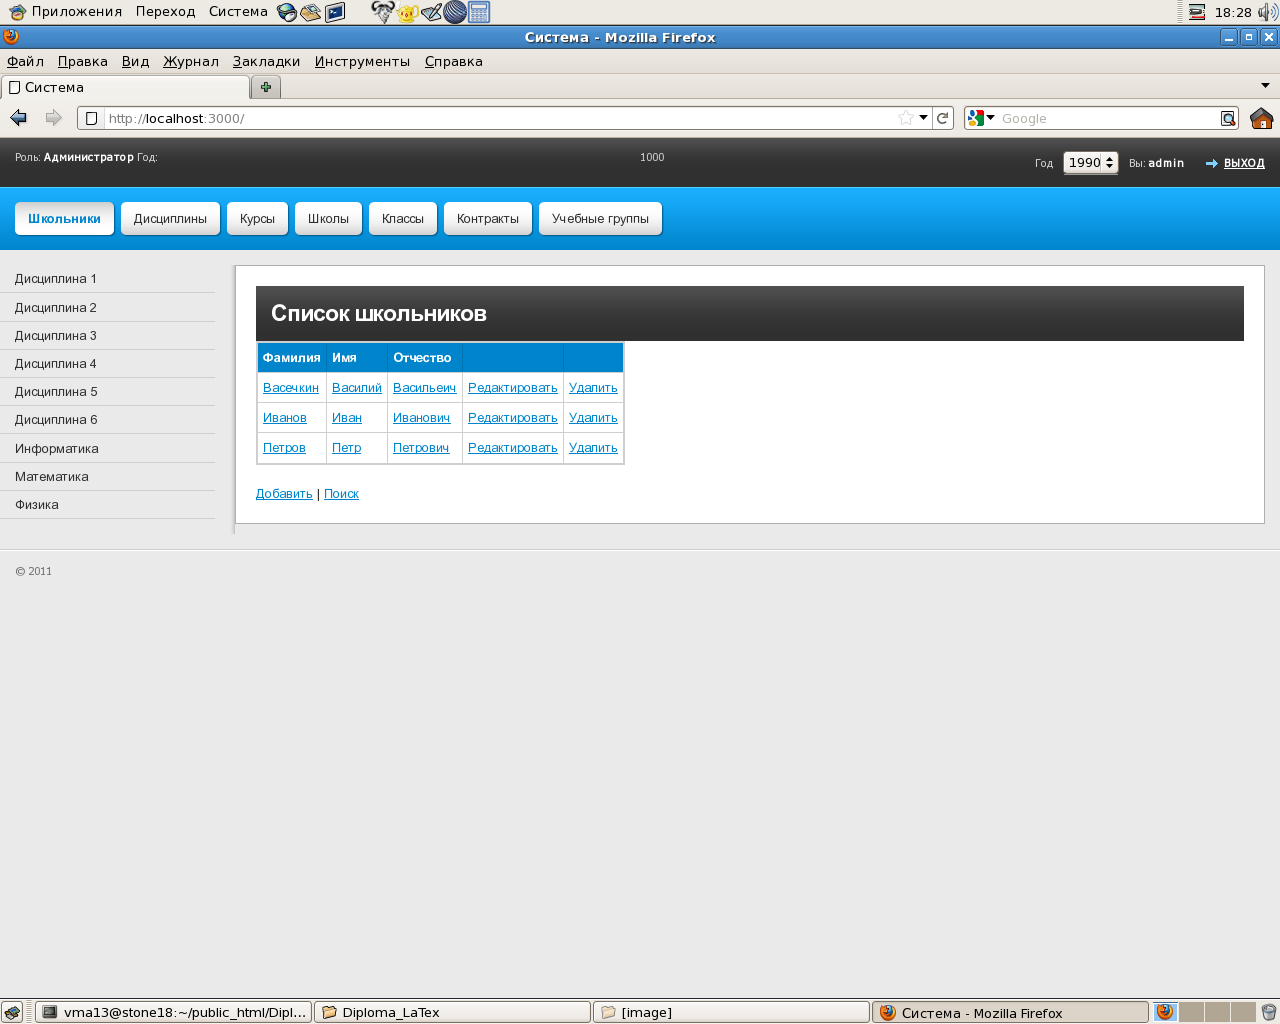
\includegraphics[scale=0.35]{image/main.png}
\end{center}
\newpage
\caption{Домашняя страничка}
\end{figure}
\newpage
Далее рассматривается, как будет выглядеть интерфейс просмотра классов, курсов, дисциплин, групп, учеников и школ.\\
\begin{figure}
\begin{center}
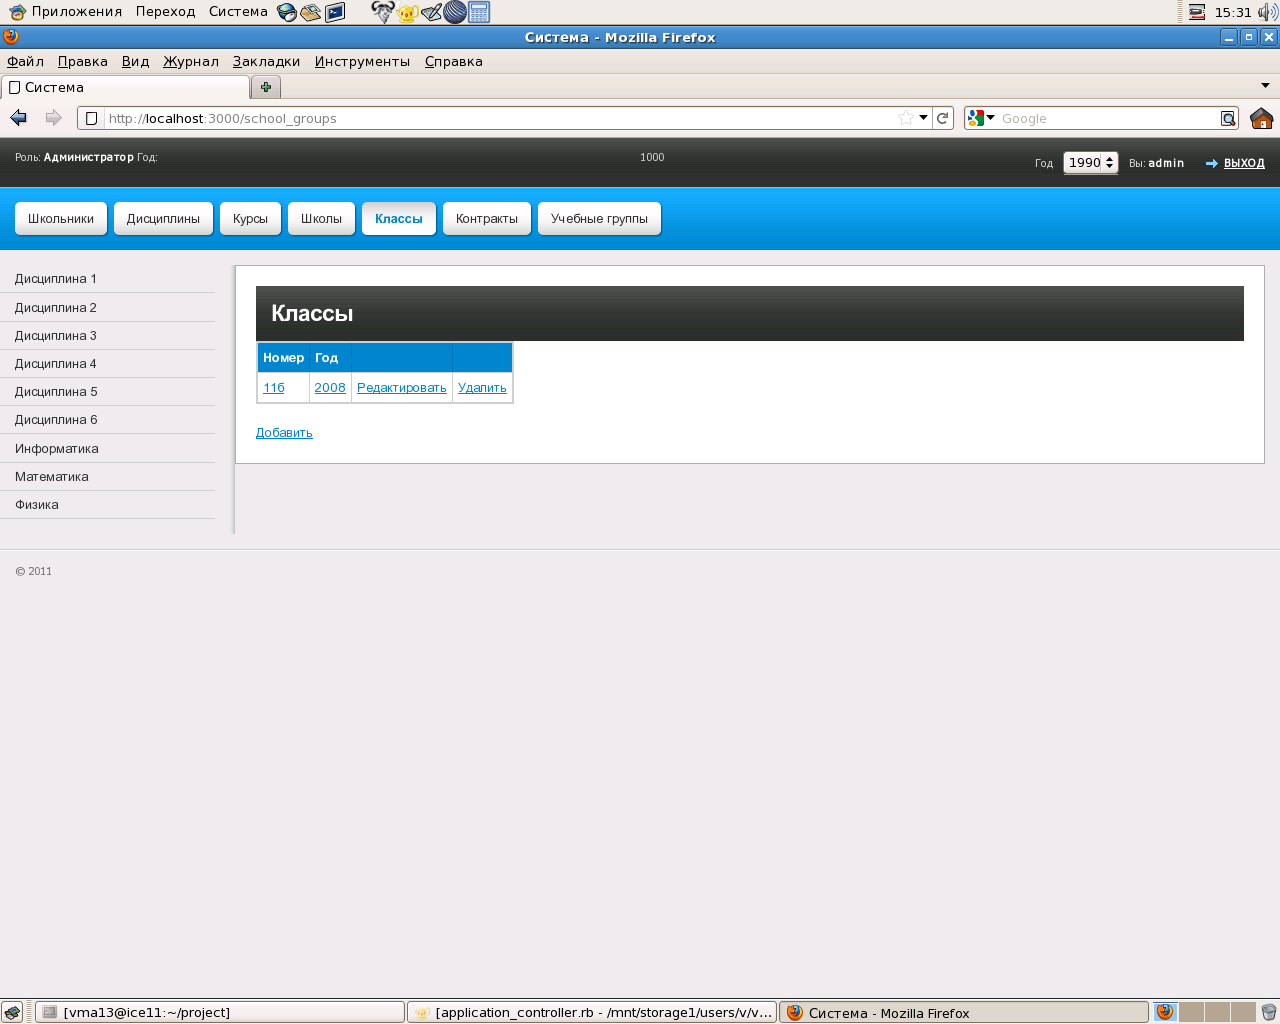
\includegraphics[scale=0.25]{image/classes.png}
\caption{Таблица школьных классов слушателей ФДО}
\end{center}
\end{figure}

\begin{figure}
\begin{center}
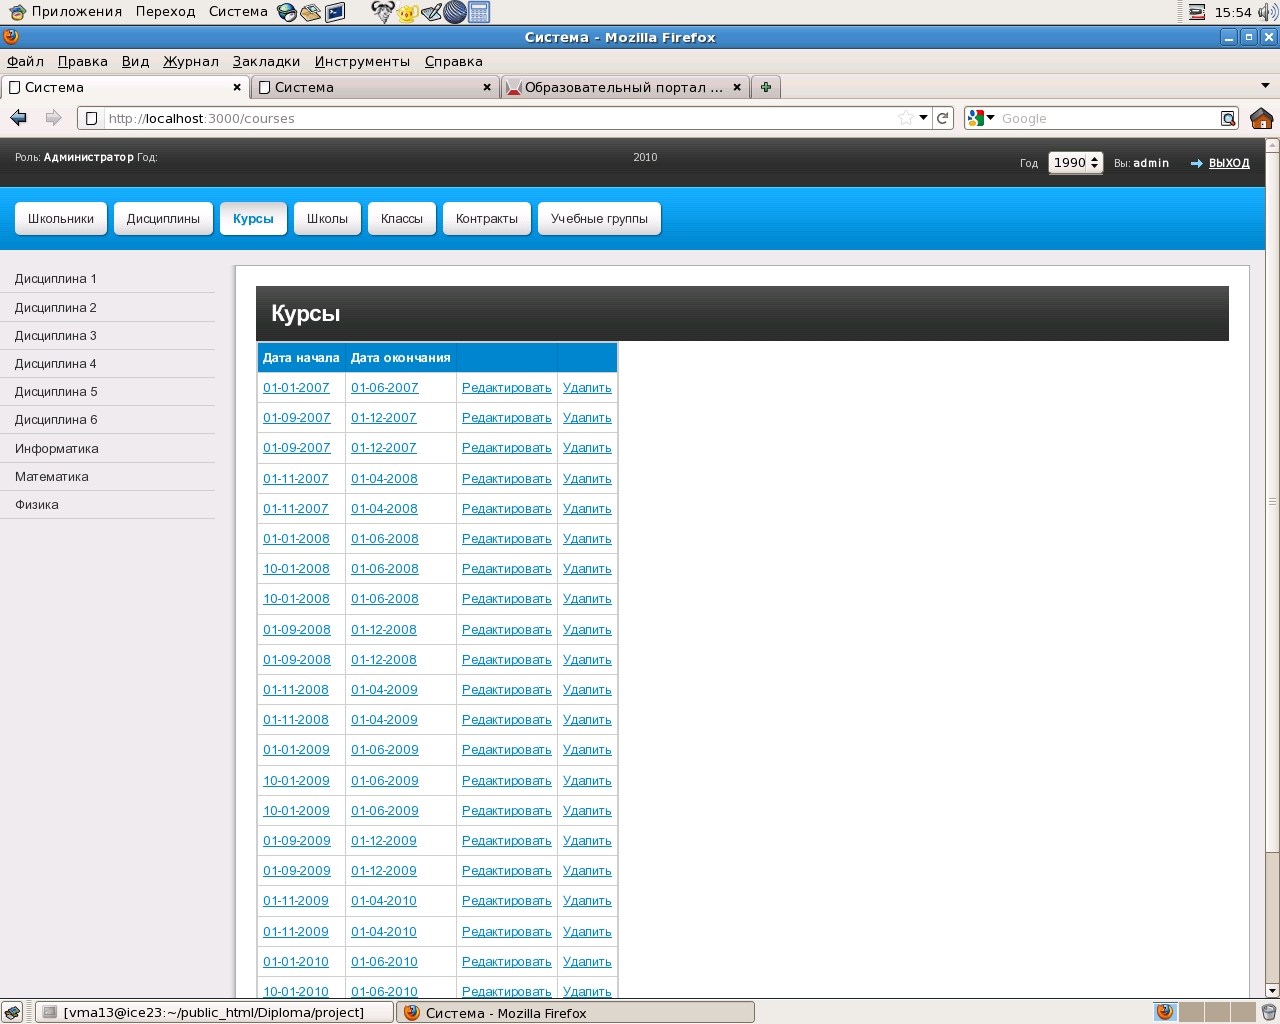
\includegraphics[scale=0.25]{image/cources.png}
\caption{Таблица курсов слушателей ФДО}
\end{center}
\end{figure}

\begin{figure}
\begin{center}
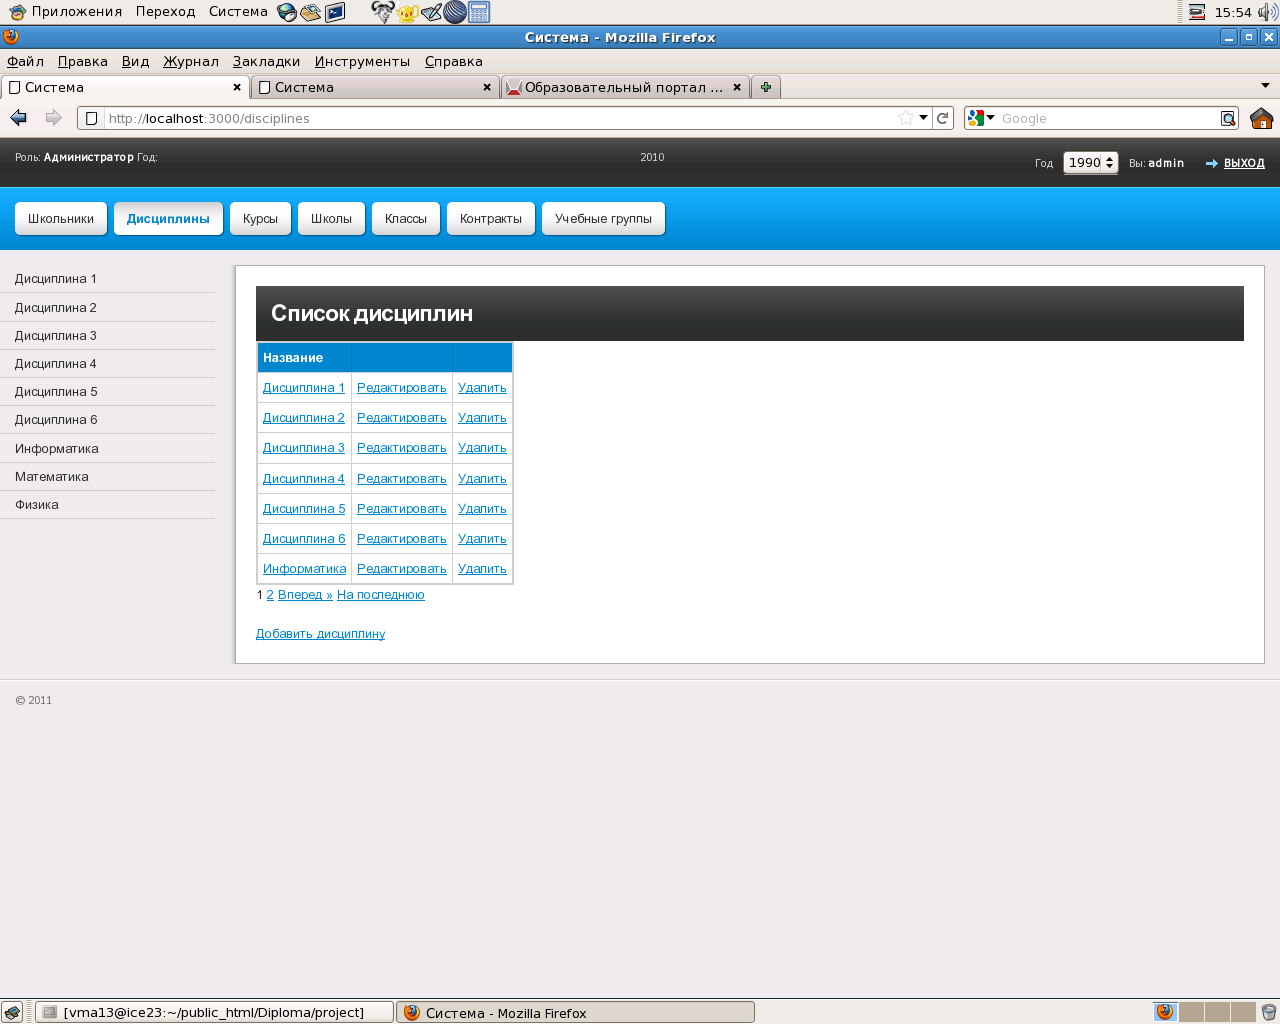
\includegraphics[scale=0.25]{image/disciplines.png}
\caption{Таблица дисциплин слушателей ФДО}
\end{center}
\end{figure}

\begin{figure}
\begin{center}
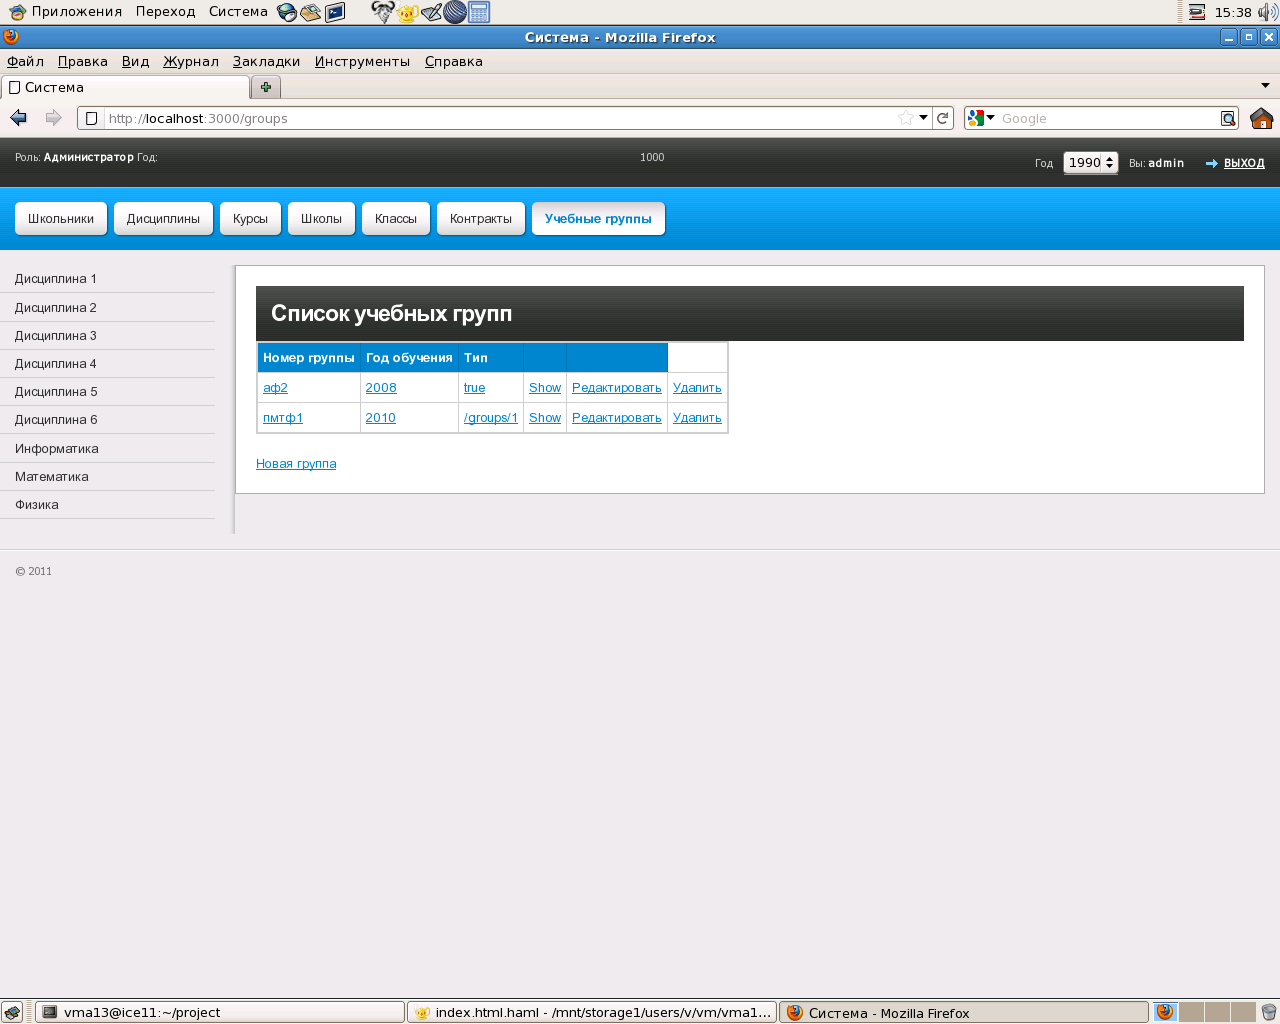
\includegraphics[scale=0.25]{image/groups.png}
\caption{Таблица групп слушателей ФДО}
\end{center}
\end{figure}


\begin{figure}
\begin{center}
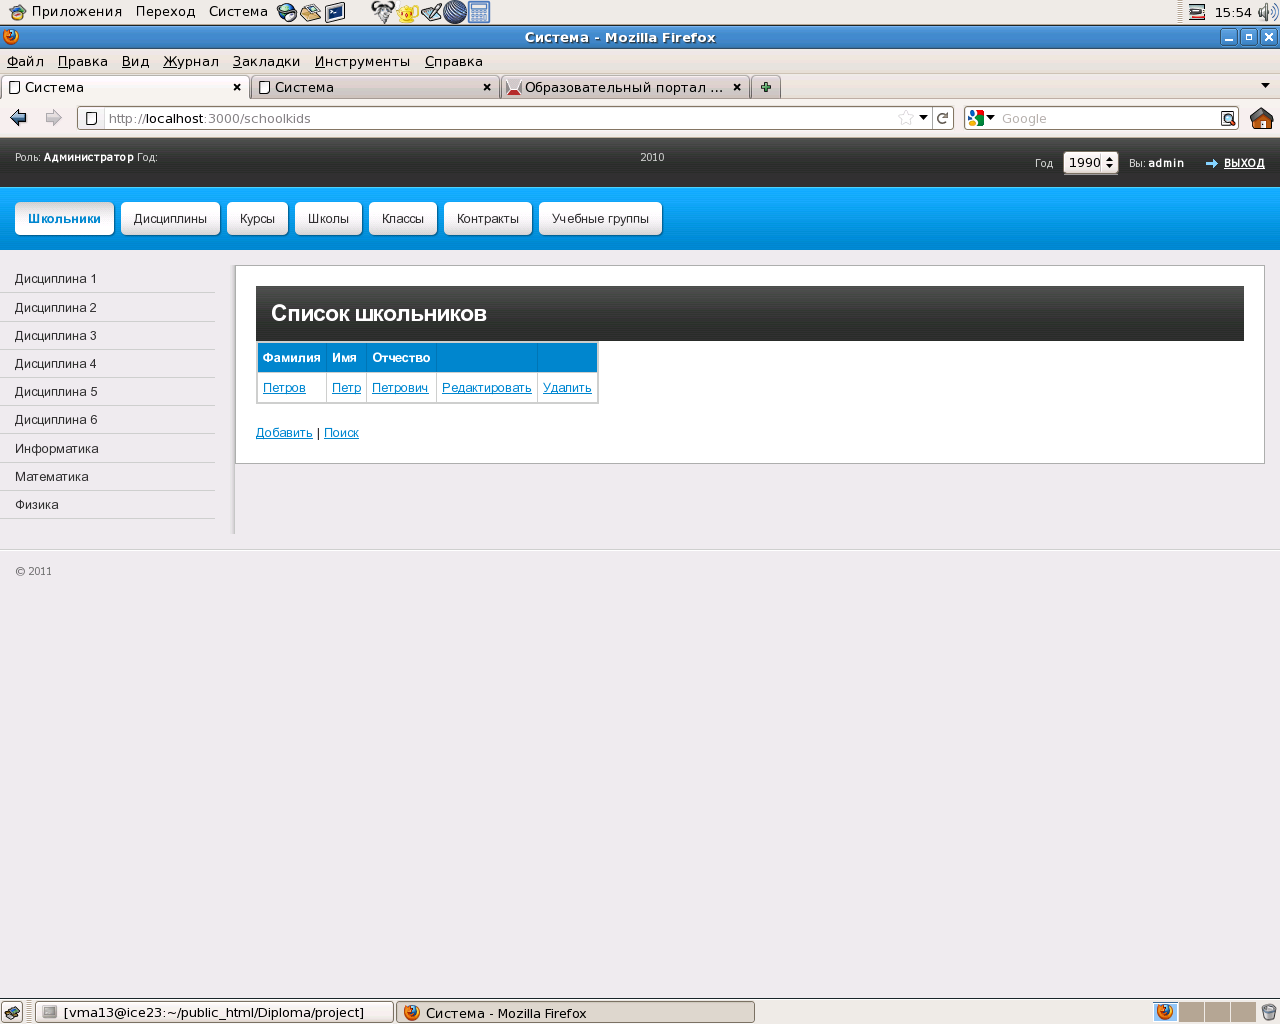
\includegraphics[scale=0.25]{image/schoolers.png}
\caption{Таблица учеников слушателей ФДО}
\end{center}
\end{figure}

\begin{figure}
\begin{center}
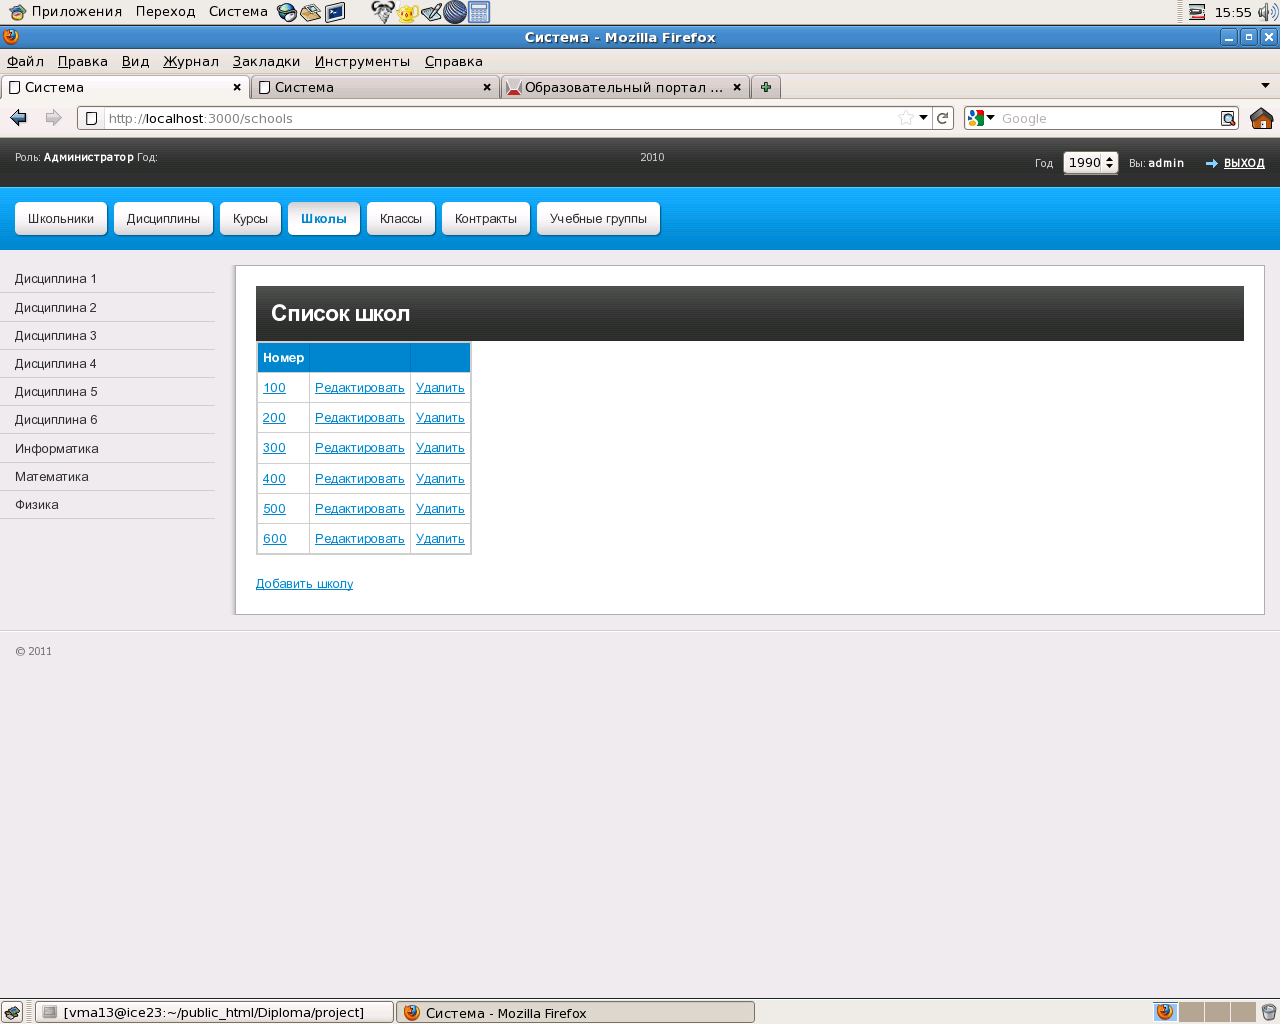
\includegraphics[scale=0.25]{image/schools.png}
\caption{Таблица школ}
\end{center}
\end{figure}

Приведем пример добавления нового учебного класса новый альбом, для этого достаточно перейти по ссылке <<Добавить>>. При нажатии на данную ссылку произойдет перенаправление на страничку создания учебного класса.\\

\begin{figure}
\begin{center}
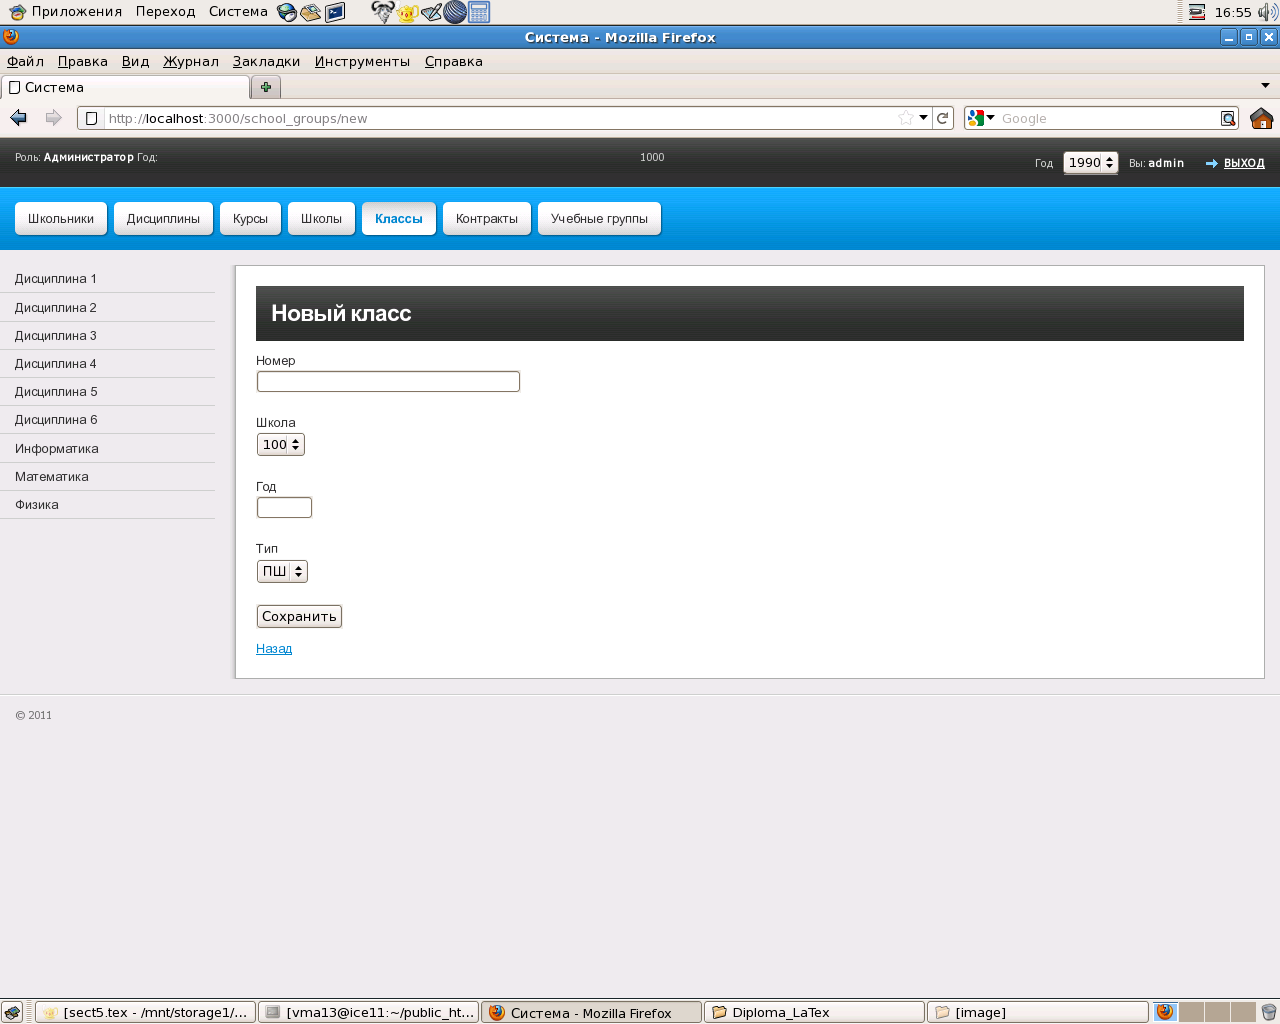
\includegraphics[scale=0.25]{image/class_new.png}
\caption{Добавление учебного класса}
\end{center}
\end{figure}

Если просто нажать кнопку <<Сохранить>>, то отобразится сообщение об ошибке.\\

\begin{figure}
\begin{center}
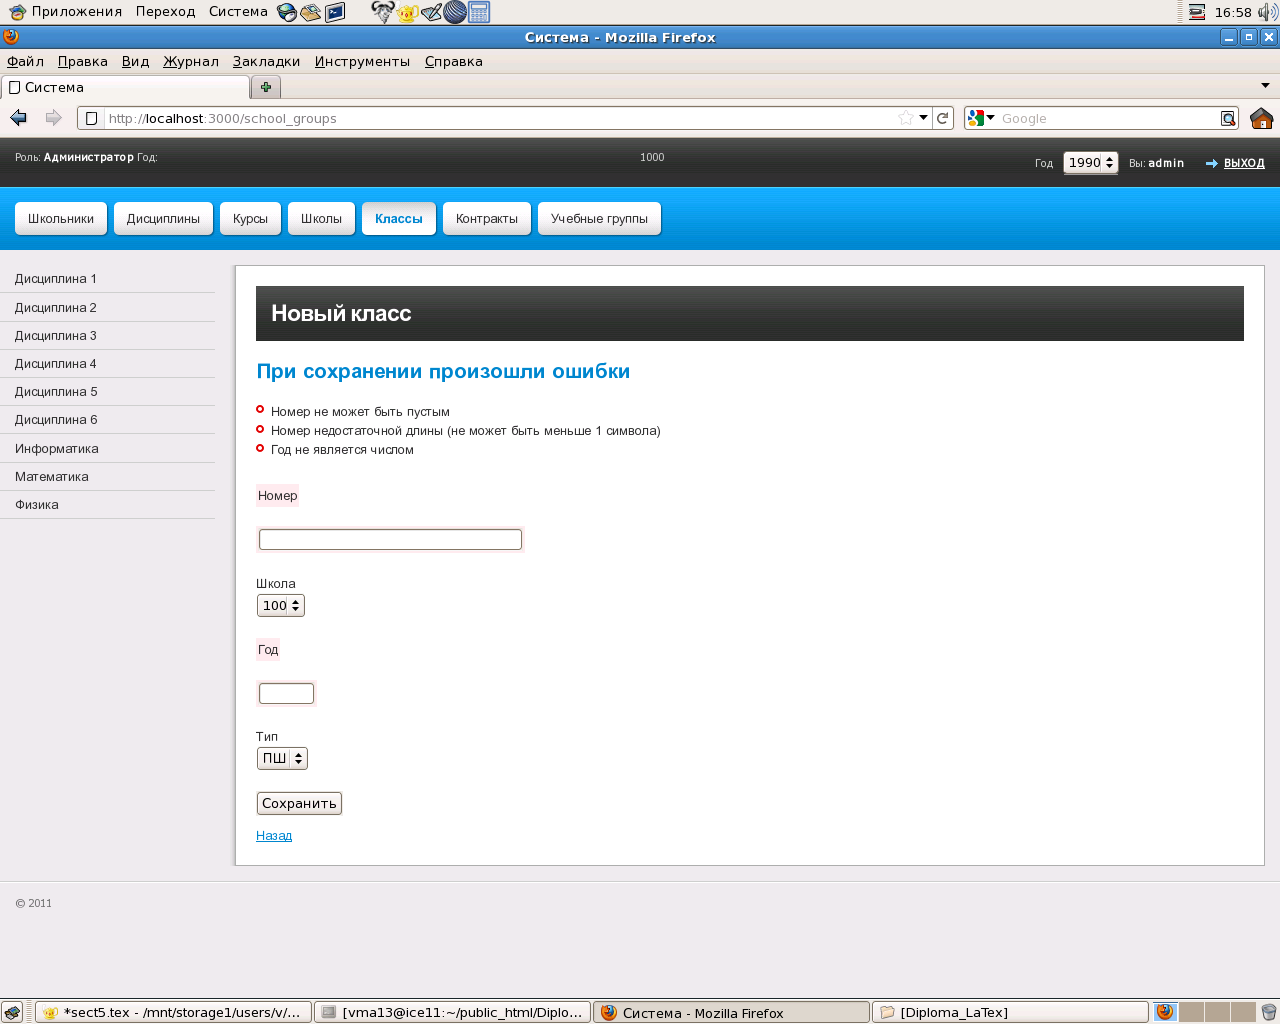
\includegraphics[scale=0.25]{image/class_error.png}
\caption{Ошибка}
\end{center}
\end{figure}

В данном случае продемонстрирован наглядный пример работы валидатора: название класса должно существовать, т.е. не существует класса без названия и это название должно содержать не менее 1 символа в названии. А также учебный год обязательно должен быть числом.\\
В остальных классах реализован аналогичный интерфейс, вот иллюстрация его работы, на примере ученика.\\

\begin{figure}[ht]
\begin{center}
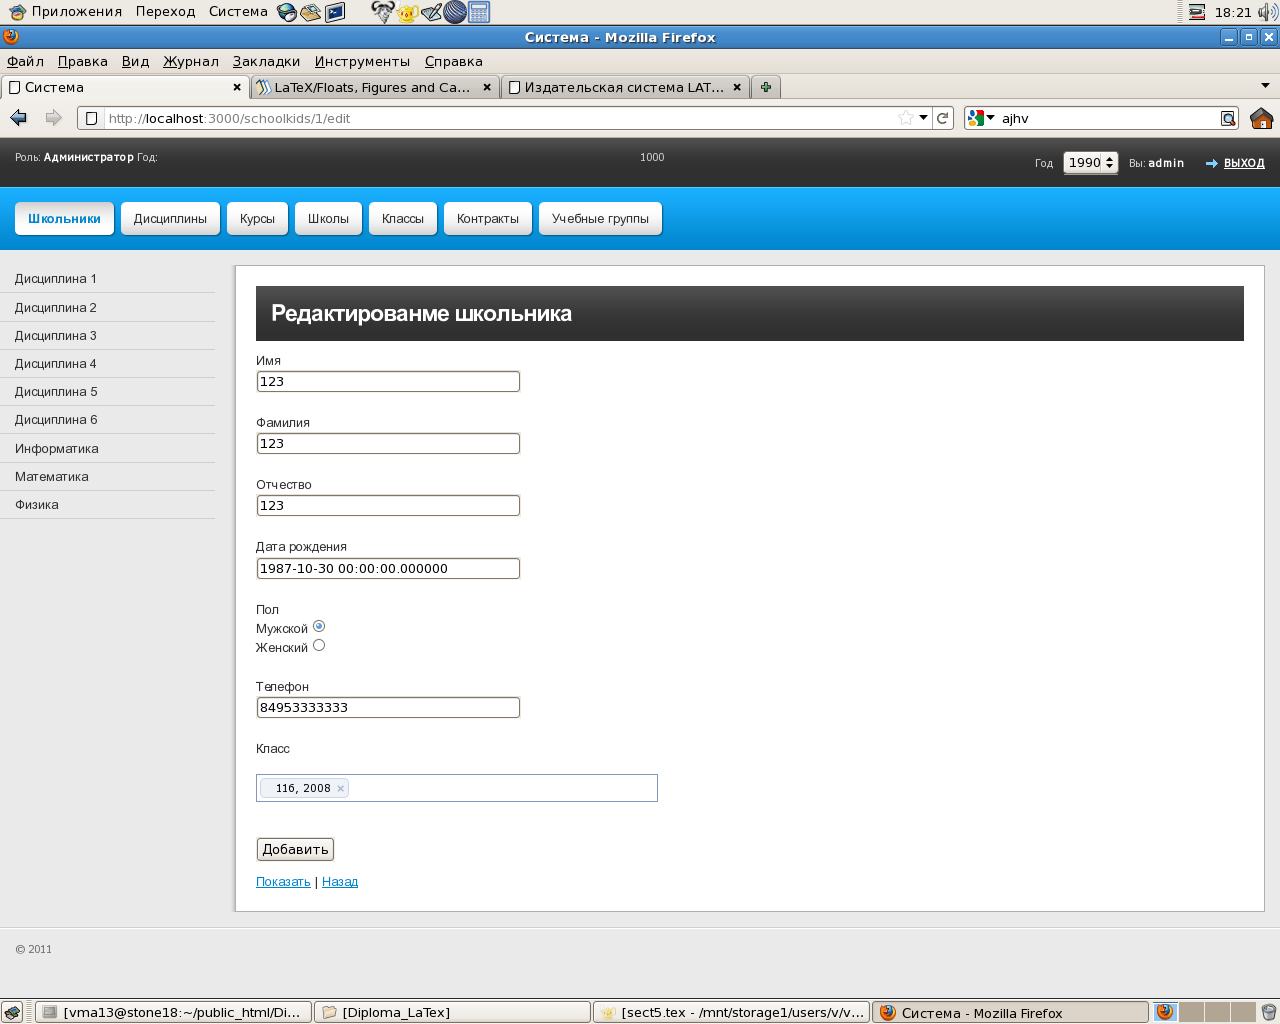
\includegraphics[scale=0.28]{image/schooler_edit.png}
\caption{Редактирование ученика}
\end{center}
\end{figure}

\begin{figure}[ht]
\begin{center}
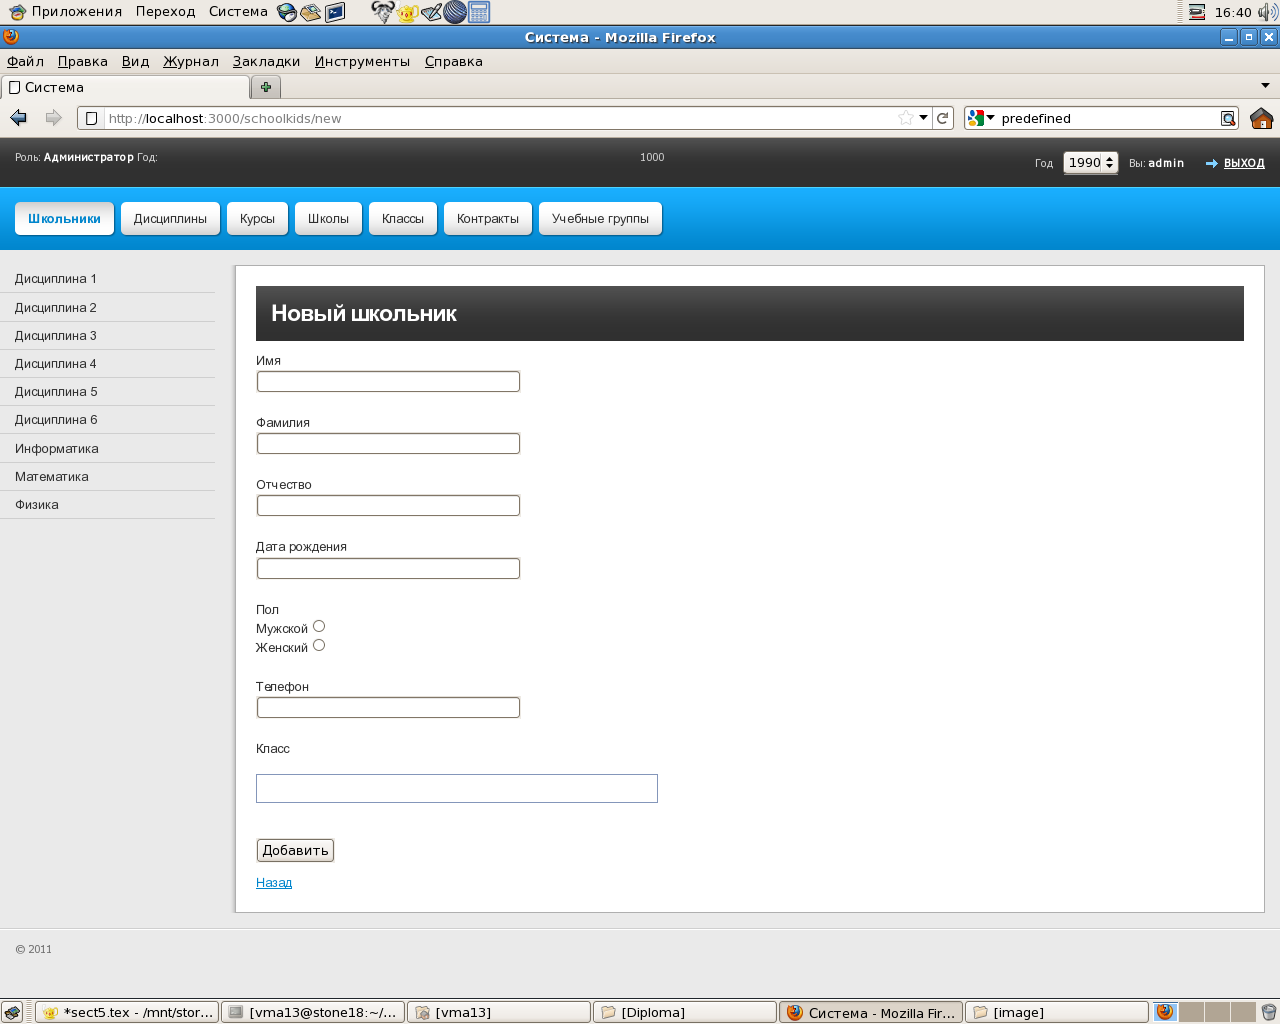
\includegraphics[scale=0.28]{image/schooler_new.png}
\caption{Создание нового ученика}
\end{center}
\end{figure}

\begin{figure}[ht]
\begin{center}
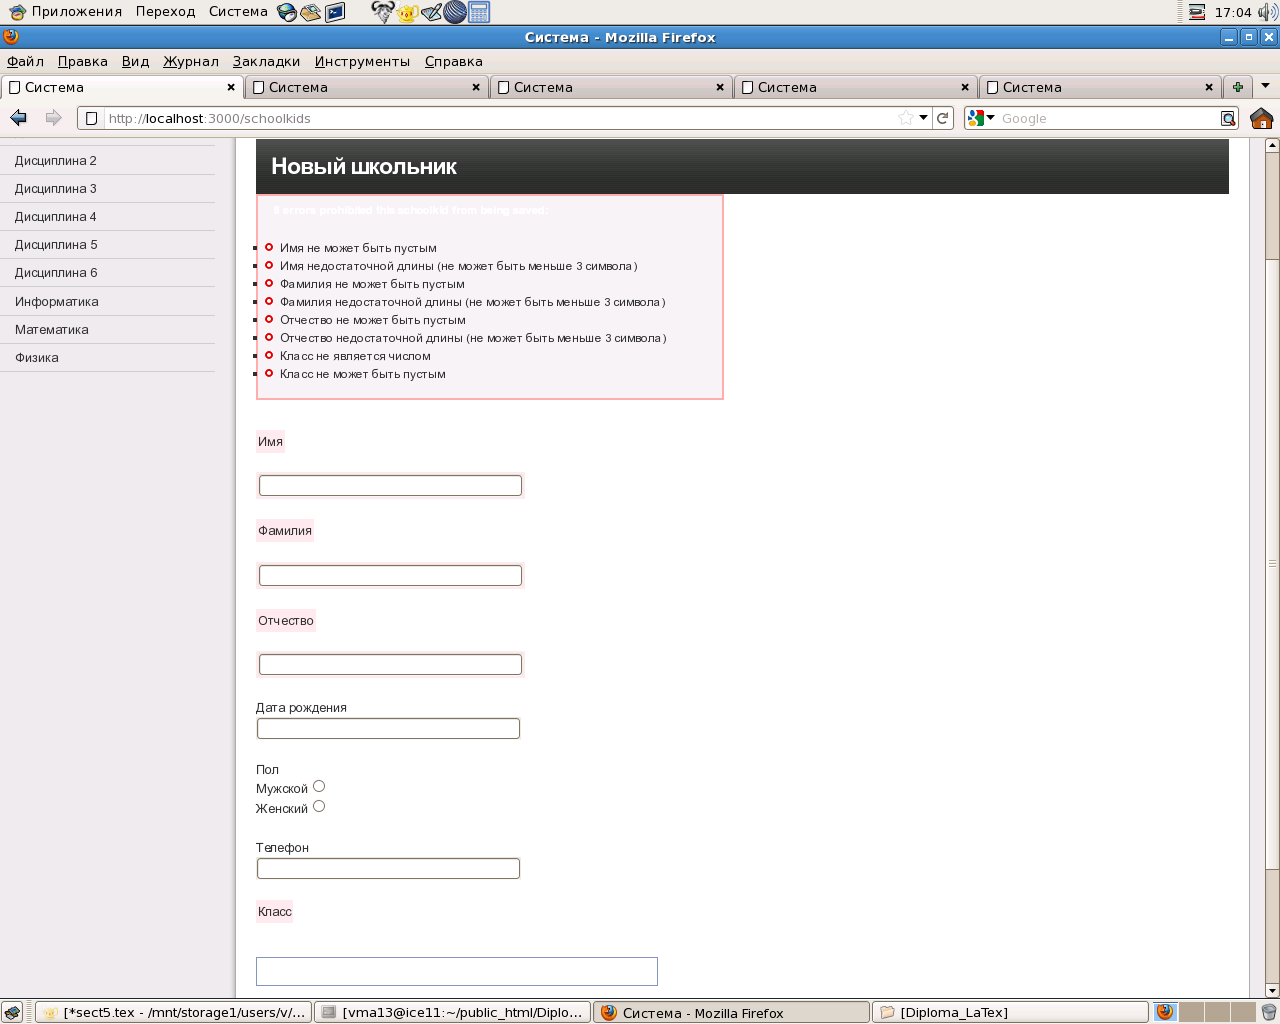
\includegraphics[scale=0.35]{image/schooler_error.png}
\caption{Ошибки при сохранении ученика}
\end{center}
\end{figure}
\endinput
